\documentclass[a4paper,12pt]{report}            % [forma A4, taille police] {Type}
    \usepackage[utf8]{inputenc}                
    \usepackage[T1]{fontenc}                        % Codage des fontes TeX
    \usepackage[francais]{babel}
    \usepackage{graphicx}
    \usepackage{wrapfig}
    \usepackage{fancyhdr}
    \usepackage{xcolor}
    \usepackage{hyperref}
    \usepackage{listings}
    \usepackage{fullpage}
    \usepackage{eso-pic}
    \usepackage{titlesec}
    \titleformat{\chapter}[hang]{\bf\huge}{\thechapter}{2pc}{}
    \lstset {numbers=left ,stepnumber=1,firstnumber=0,numberfirstline=true}
    \hypersetup{
        bookmarks=true,         % show bookmarks bar?
        unicode=false,          % non-Latin characters in Acrobat’s bookmarks
        pdftoolbar=true,        % show Acrobat’s toolbar?
        pdfmenubar=true,        % show Acrobat’s menu?
        pdffitwindow=false,     % window fit to page when opened
        pdfstartview={FitH},    % fits the width of the page to the window
        pdftitle={My title},    % title
        pdfauthor={Author},     % author
        pdfsubject={Subject},   % subject of the document
        pdfcreator={Creator},   % creator of the document
        pdfproducer={Producer}, % producer of the document
        pdfkeywords={keyword1, key2, key3}, % list of keywords
        pdfnewwindow=true,      % links in new PDF window
        colorlinks=true,       % false: boxed links; true: colored links
        linkcolor=black,          % color of internal links (change box color with linkbordercolor)
        citecolor=green,        % color of links to bibliography
        filecolor=magenta,      % color of file links
        urlcolor=blue           % color of external links
    }
    
    \author{Samuel HUET \& Thomas COUTANT}
    \title{\huge{Les Antennes}}
    
    \begin{document}
\maketitle
\renewcommand{\contentsname}{SOMMAIRE} % Dans le corps du document,avant la commande \tableofcontents.
\tableofcontents

\chapter{Amplificateur}
\addcontentsline{toc}{chapter}{Amplificateur}

\section{Pertes}

Avant de pouvoir déterminer l'amplification de l'amplificateur, il est nécéssaire de déterminer la pertude dûs aux cables, 
Pour cela, nous utilisons le montage suivant :

\begin{center}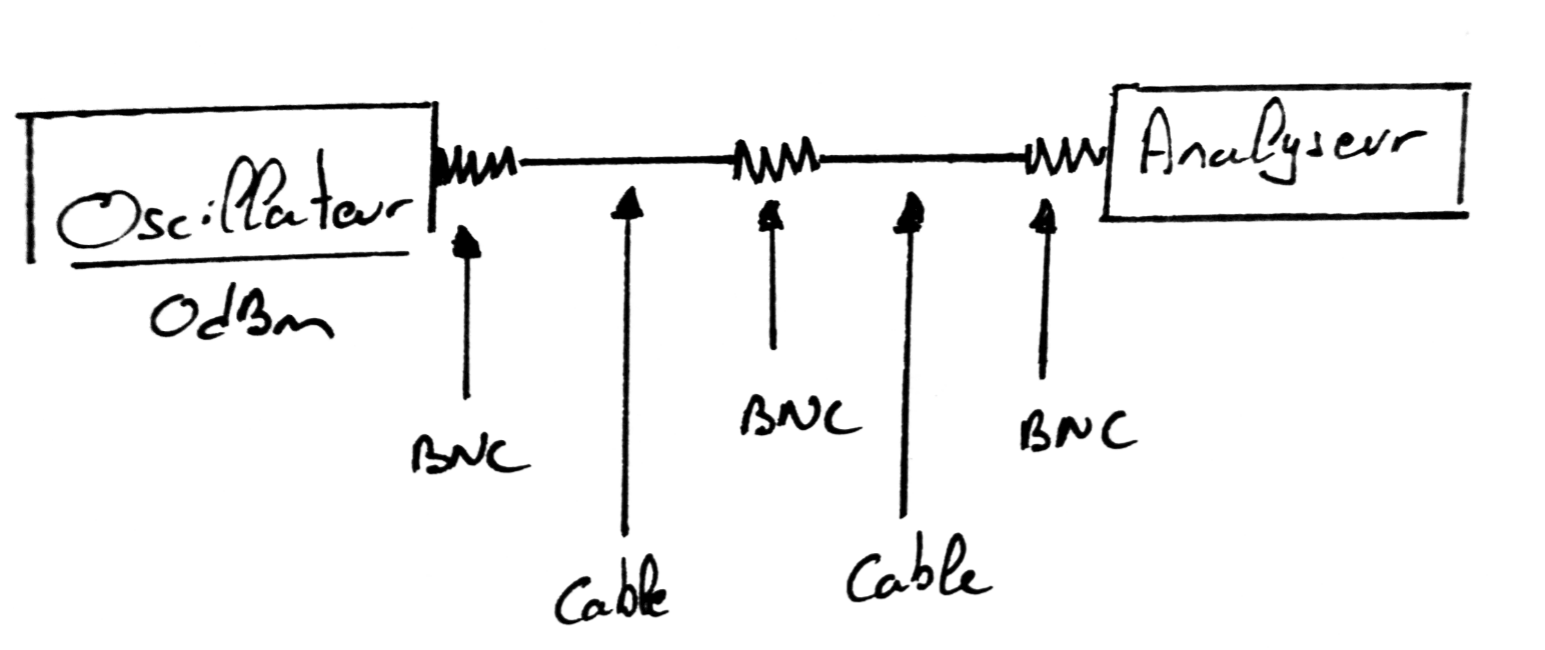
\includegraphics[scale = 0.2]{pic/mesure_perte.png}\\ \end{center}

Il est ainsi très facile, en visualisant l'analyseur de spectre de derterminer ces pertes.
Sur notre exemple, avec les cables coaxiaux utlisés, la perte de 4.2 dB, mais cela dépend évidemment du type de
materiel utilisé. Cette mesure sera donc à prendre en compte pour chaque relevé.

\section{Gain}

Afin de déterminer sa valeur d'amplification, le but est de le faire fonctionner. La puissance d'entrée étant
connue, ainsi que les pertes dû aux cables, il suffira alors d'observer la puissance recu sur
l'analyseur de spectre.

\begin{center}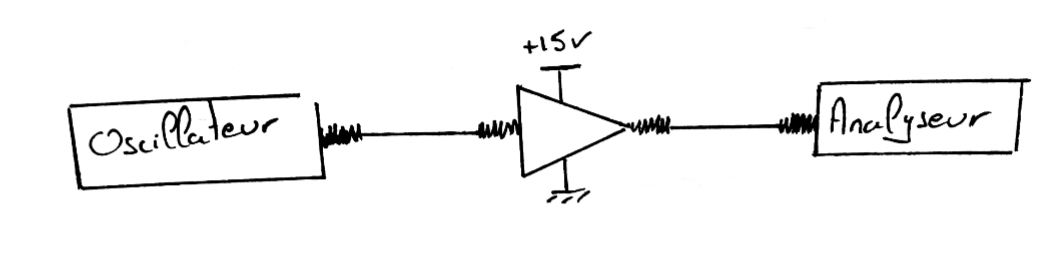
\includegraphics[scale = 0.3]{pic/montage_ampli.png}\\ \end{center}

Nous avons, avec l'oscillateur, généré un signal de 220 MHz à -15 dBm (Attention à ne pas monter trop haut, en 
effet, si l'amplificateur sature, la mesure est entièrement faussé. -15dBm est une puissance assez basse mais il
serait prudent de réaliser plusieurs fois la mesure avec des puissances d'entré différentes pour être sûr de 
la mesure.

A la sortie, nous avons donc 9.6dBm sur la fréquence 220MHz. En ajoutant les 4.2dBm de pertes sur la ligne, nous arrivons
à 13.8 dBm en sortie. La différence étant de 28.6 dB, nous pouvons en conclure qu'il s'agit là du gain de l'amplificateur.
Il faut alors la convertir en valeur linéaire :\\
$$10 \log (x) = 28.6 dB$$
$$\Rightarrow x = 10^{\frac{28.6}{10}}=724.4 $$

\chapter{WattMètre}
\addcontentsline{toc}{chapter}{WattMètre}

Le WattMètre permet de nous donner le ROS (Rapport d'onde stationaire), mais aussi le FWD (l'onde incidente) et le
RFL (l'onde réfléchis). Cependant, il ne fonctionne que dans une certaine gamme de puissance. Ici, la puissance minimal
à l'entrée est de 0.3W (=24.7dBm). Nous devons alors calculer quelle puissance il faudra rentrer sur l'oscillateur.

\begin{center}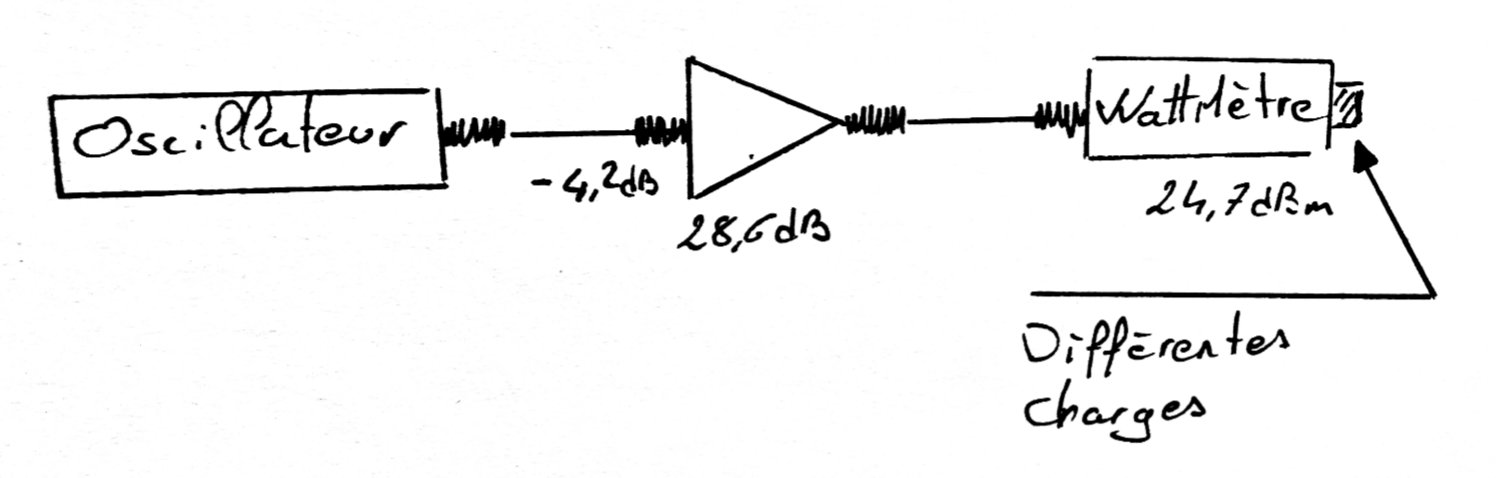
\includegraphics[scale = 0.25]{pic/montage_wattmetre.png}\\ \end{center}

Nous avons donc l'équation : $x+28.6-4.2=24.7$. Il faudra alors au moins avoir une puissance de sortie de 0.3dBm.
Nous avons alors procédé aux 3 mesures que permettait le wattmètre en y branchant différentes charge : 50$\Omega$ ,un court-circuit (0$\Omega$), et un circuit ouvert (impédance infinie).
Notre ligne étant addapté pour 50$\Omega$, nous nous attendons à vois un ROS faible pour la charge 50$\Omega$. Voici les 
résultats obtenues :

\begin{center}
	\begin{tabular}{||p{4cm}||*{4}{c|}|}
		\hline
		\bfseries         & 50$\Omega$ & CC              & CO       & Charge inconnue \\
		\hline
		\hline
		\bfseries SWR     & 1.71       & 15.7 ($\infty$) & $\infty$ & 3.74            \\
		\hline
		\bfseries FWD (W) & 0.330      & 0.336           & 0.210    & 0.283           \\
		\hline
		\bfseries RFL (W) & 0.022      & 0.262           & 0.215    & 0.095           \\
		\hline
		\hline
	\end{tabular}
\end{center}

Afin de trouver la charge inconnue, il existe deux formules liant charge et SWR :
\begin{itemize}
	\item $\mbox{SWR} = \frac{Z_{souce}}{Z_{charge}}$
	\item $\mbox{SWR} = \frac{Z_{charge}}{Z_{souce}}$
\end{itemize}

C'est la seconde que l'on va utiliser ici, car elle nous donne la formule suivante : 
$Z_{charge} = \mbox{SWR} \cdot Z_{source} = 187\Omega$
Ce qui correspond au code couleur de 150 $\Omega$


\chapter{Mesure d'antennes}
\addcontentsline{toc}{chapter}{Mesure d'antennes}

Afin de determiner les bandes passantes des antennes, nous pouvons mesurer le ROS de chacune d'entre elles
à différentes fréquances. La où le ROS sera inferieur à 2, nous pourrons conclure que l'antenne est 
addaptée. Mais avant cela, il serait préférable de déterminer pour quelle gammme de fréquence est taillé chaque antenne. \\
Pour cela, nous avons 2 formules :
\begin{itemize}
	\item $L = \frac{\lambda}{4}$
	\item $\lambda = \frac{c}{f}$
\end{itemize}
Sachant alors que plus l'antenne est petite, plus elle est adapté aux hautes fréquences, nous pouvons dors et
déjà supposer que la plus petite est taillée pour la UHF (300MHz - 3000MHz) et la grande, plutot pour la
VHF (30MHz - 300MHz). Voici donc les mesures de ROS pour les deux antennes ainsi que le la courbe de calcule 
du ROS en fonction de l'onde réfléchie et incidente, donnée par cette formule :
$$\mbox{SWR} = \frac{  1+ \sqrt{\frac{P_{R}}{P_{D}}  }   }{1- \sqrt{\frac{P_{R}}{P_{D}}  }}  $$

\begin{center}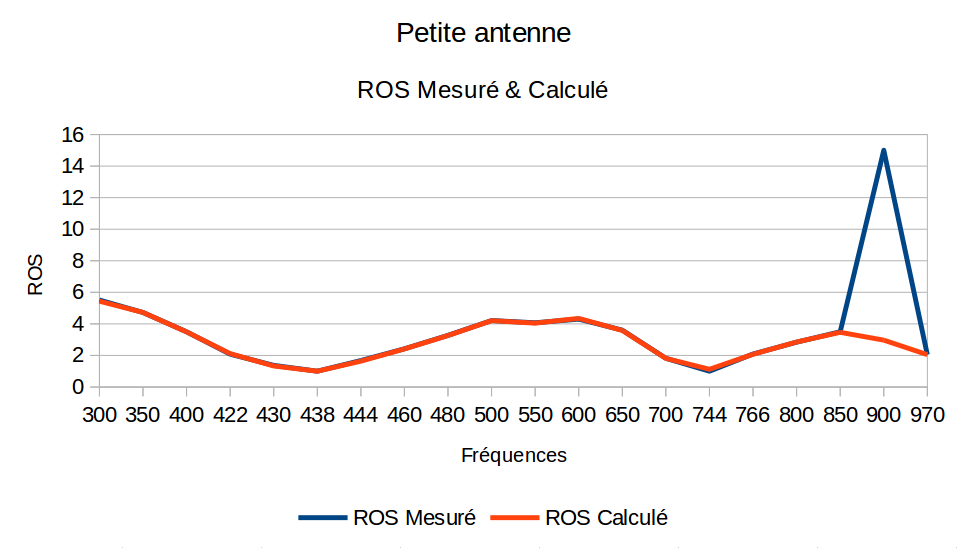
\includegraphics[scale = 0.5]{pic/ROS_petite_antenne.png}\\ \end{center}
\begin{center}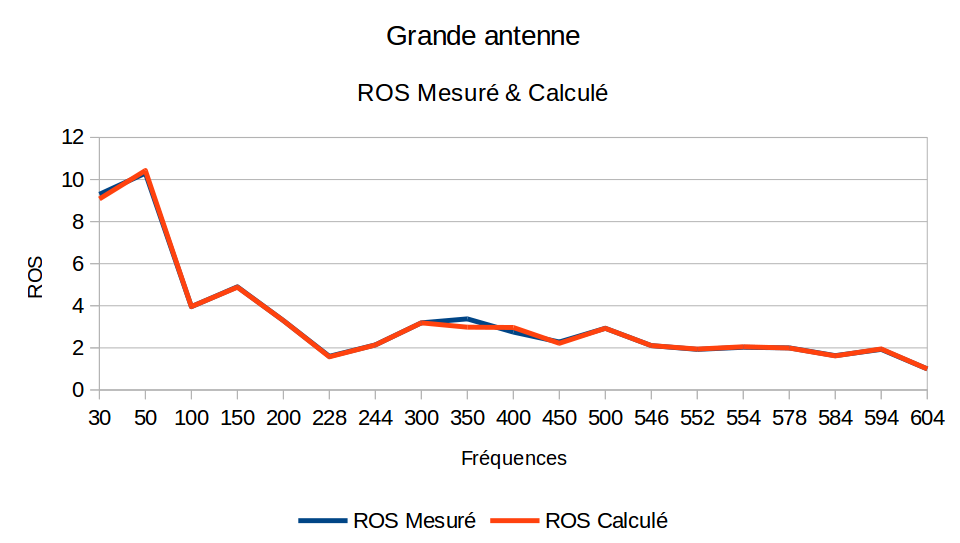
\includegraphics[scale = 0.5]{pic/ROS_grande_antenne.png}\\ \end{center}

On peut voir sur les deux courbes que les ROS mesurés et calculés se suivent avec précision, à l'exeption
d'un point sur la petite antenne, probablement lié à une erreur de mesure. Cependant, avec des courbes, il
est difficile de déterminer la fréquence de fonctionnement de ces deux antennes. Les relevés ne sont pas assez 
précis et nous devons alors utiliser une autre methode.\\
La seconde méthode consiste à utiliser un analyseur de réseau. Son but est de nous fournir une courbe des
paramètres S, et ainsi de voir en quels endroits l'antenne est la plus adaptée. Mais ce genre d'appareil nécéssite 
d'être calibré avant utilisation.

Pour cela, appuyez sur le bouton \textbf{CAL} de l'analyseur, on accède alors au menu de calibration. On selectionne
alors le port souhait puis, grâce aux standars de calibrations (50$\Omega$, CC et CO) il suffit de suivre les étapes
dicté par la machine en branchant les différentes charges au bon port. Maintenant que notre analyseur est 
calibré, nous voila près à déterminer les fréquences.

\section{Petite antenne}

\begin{center}
	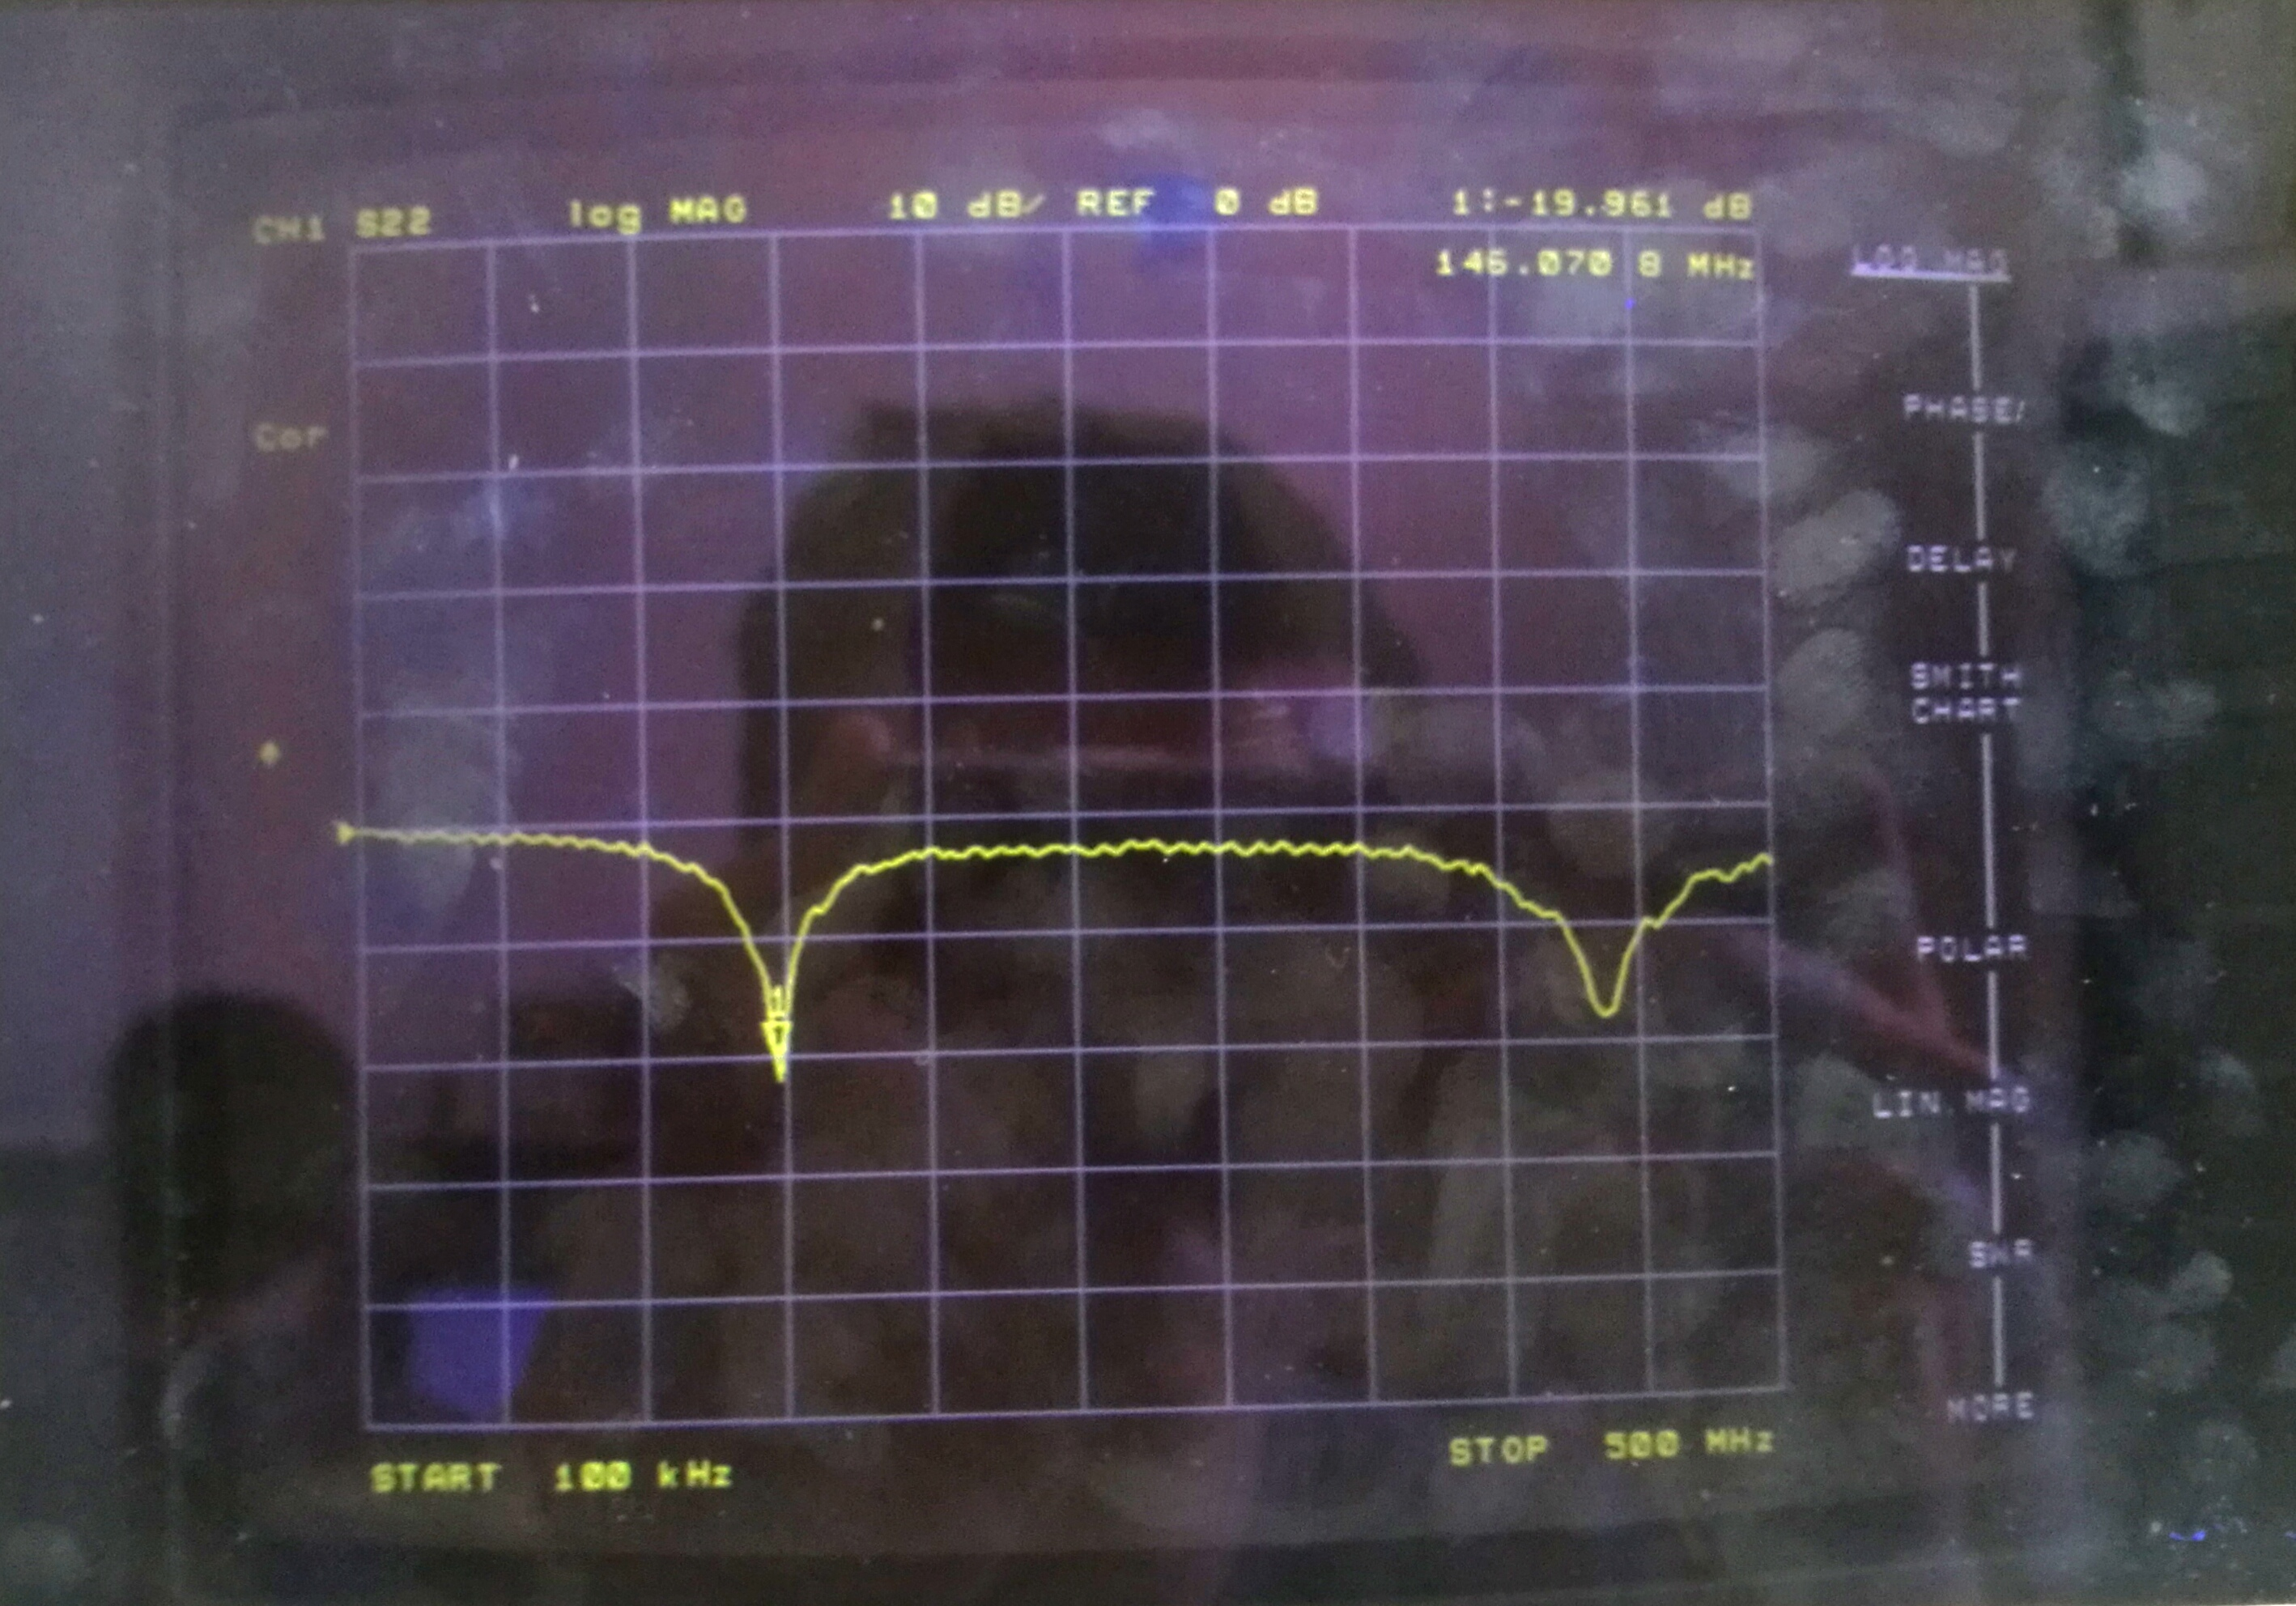
\includegraphics[scale = 0.072]{pic/S_petite.jpg}
	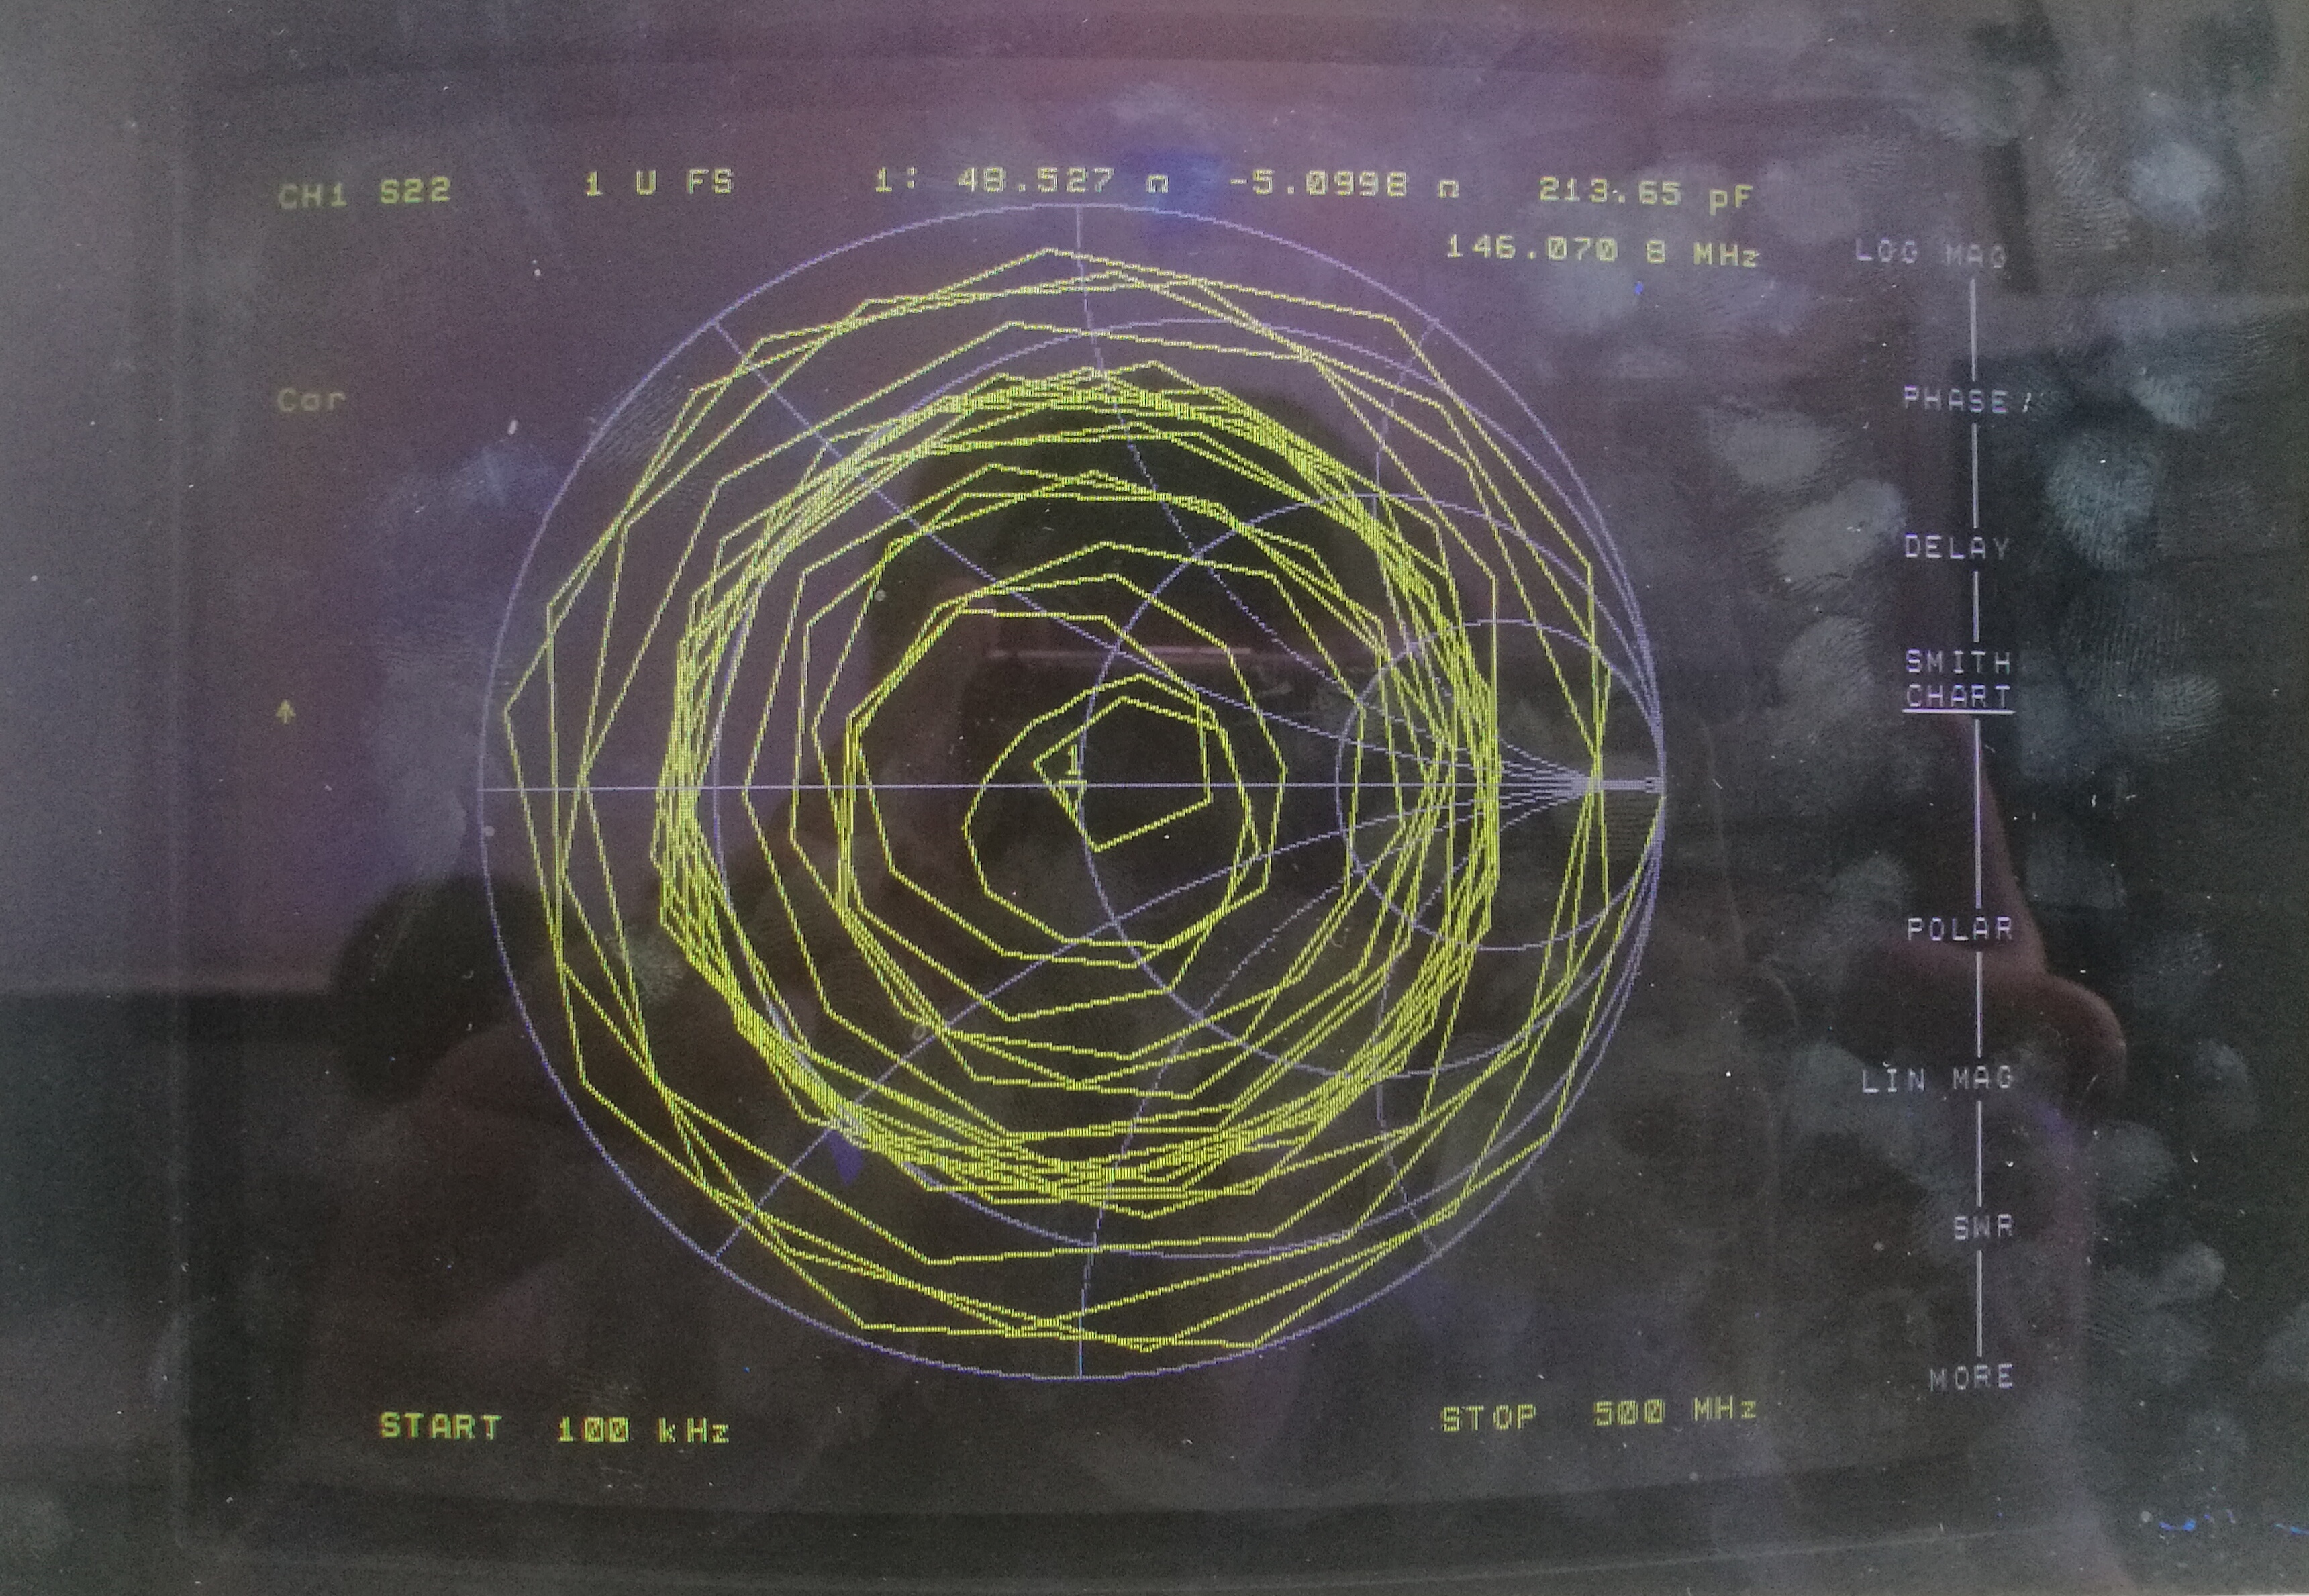
\includegraphics[scale = 0.06]{pic/Smith_petite.jpg} 
\end{center}

Nous pouvons constater que les courbes sont ainsi bien plus précises que sur les graphiques précédentes.
Et nous pouvons répérer des creux importants à 150MHz ainsi qu'à 438MHz. L'antenne ayant plutot une allure 
UHF, nous allons utiliser la fréquence 438MHz pour les cacules. 
$$ L = \frac{c}{4\cdot f} = 17cm$$

Cette valeur semble cohérente, l'antenne fait à peu près cette taille. Si en pratique elle semble 
plus petite, c'est grâce à l'inductance placé à sa base qui permet d'en réduire sa taille. Si elle 
semble plus petite, c'est que le pied n'est pas compris dans l'antenne.

\section {Grande antenne}

\begin{center}
	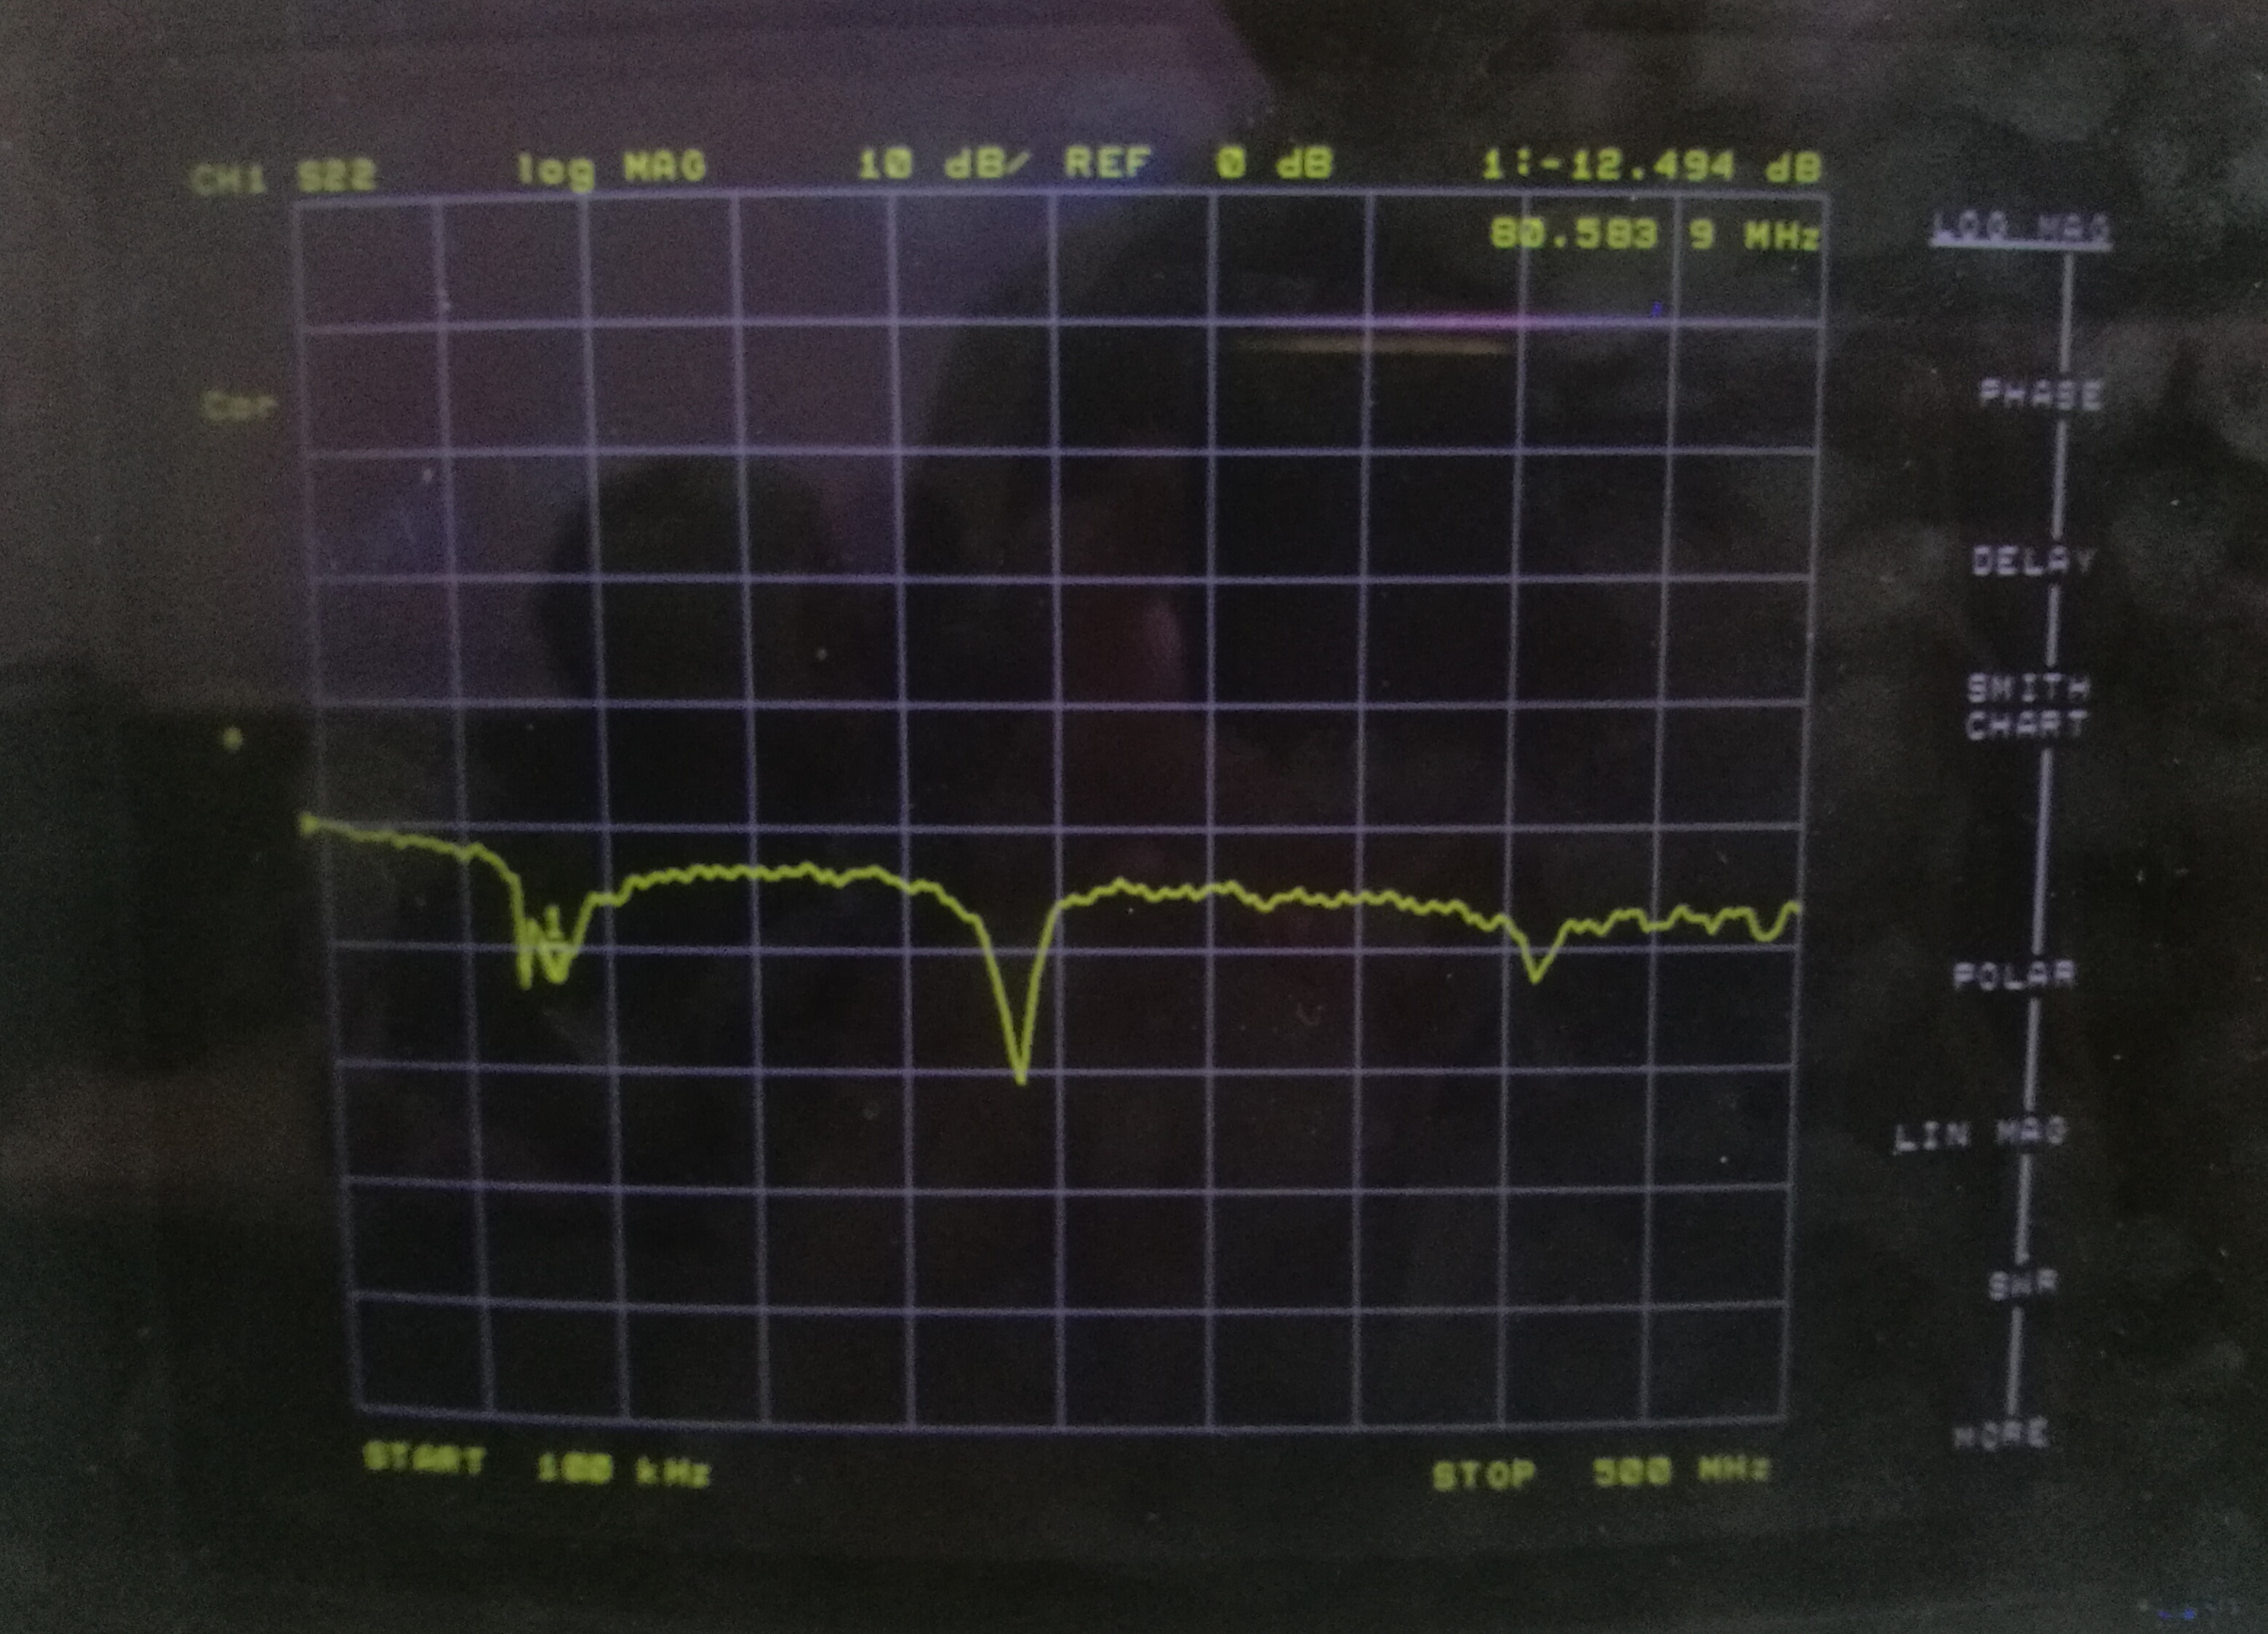
\includegraphics[scale = 0.062]{pic/S_grande.jpg}
	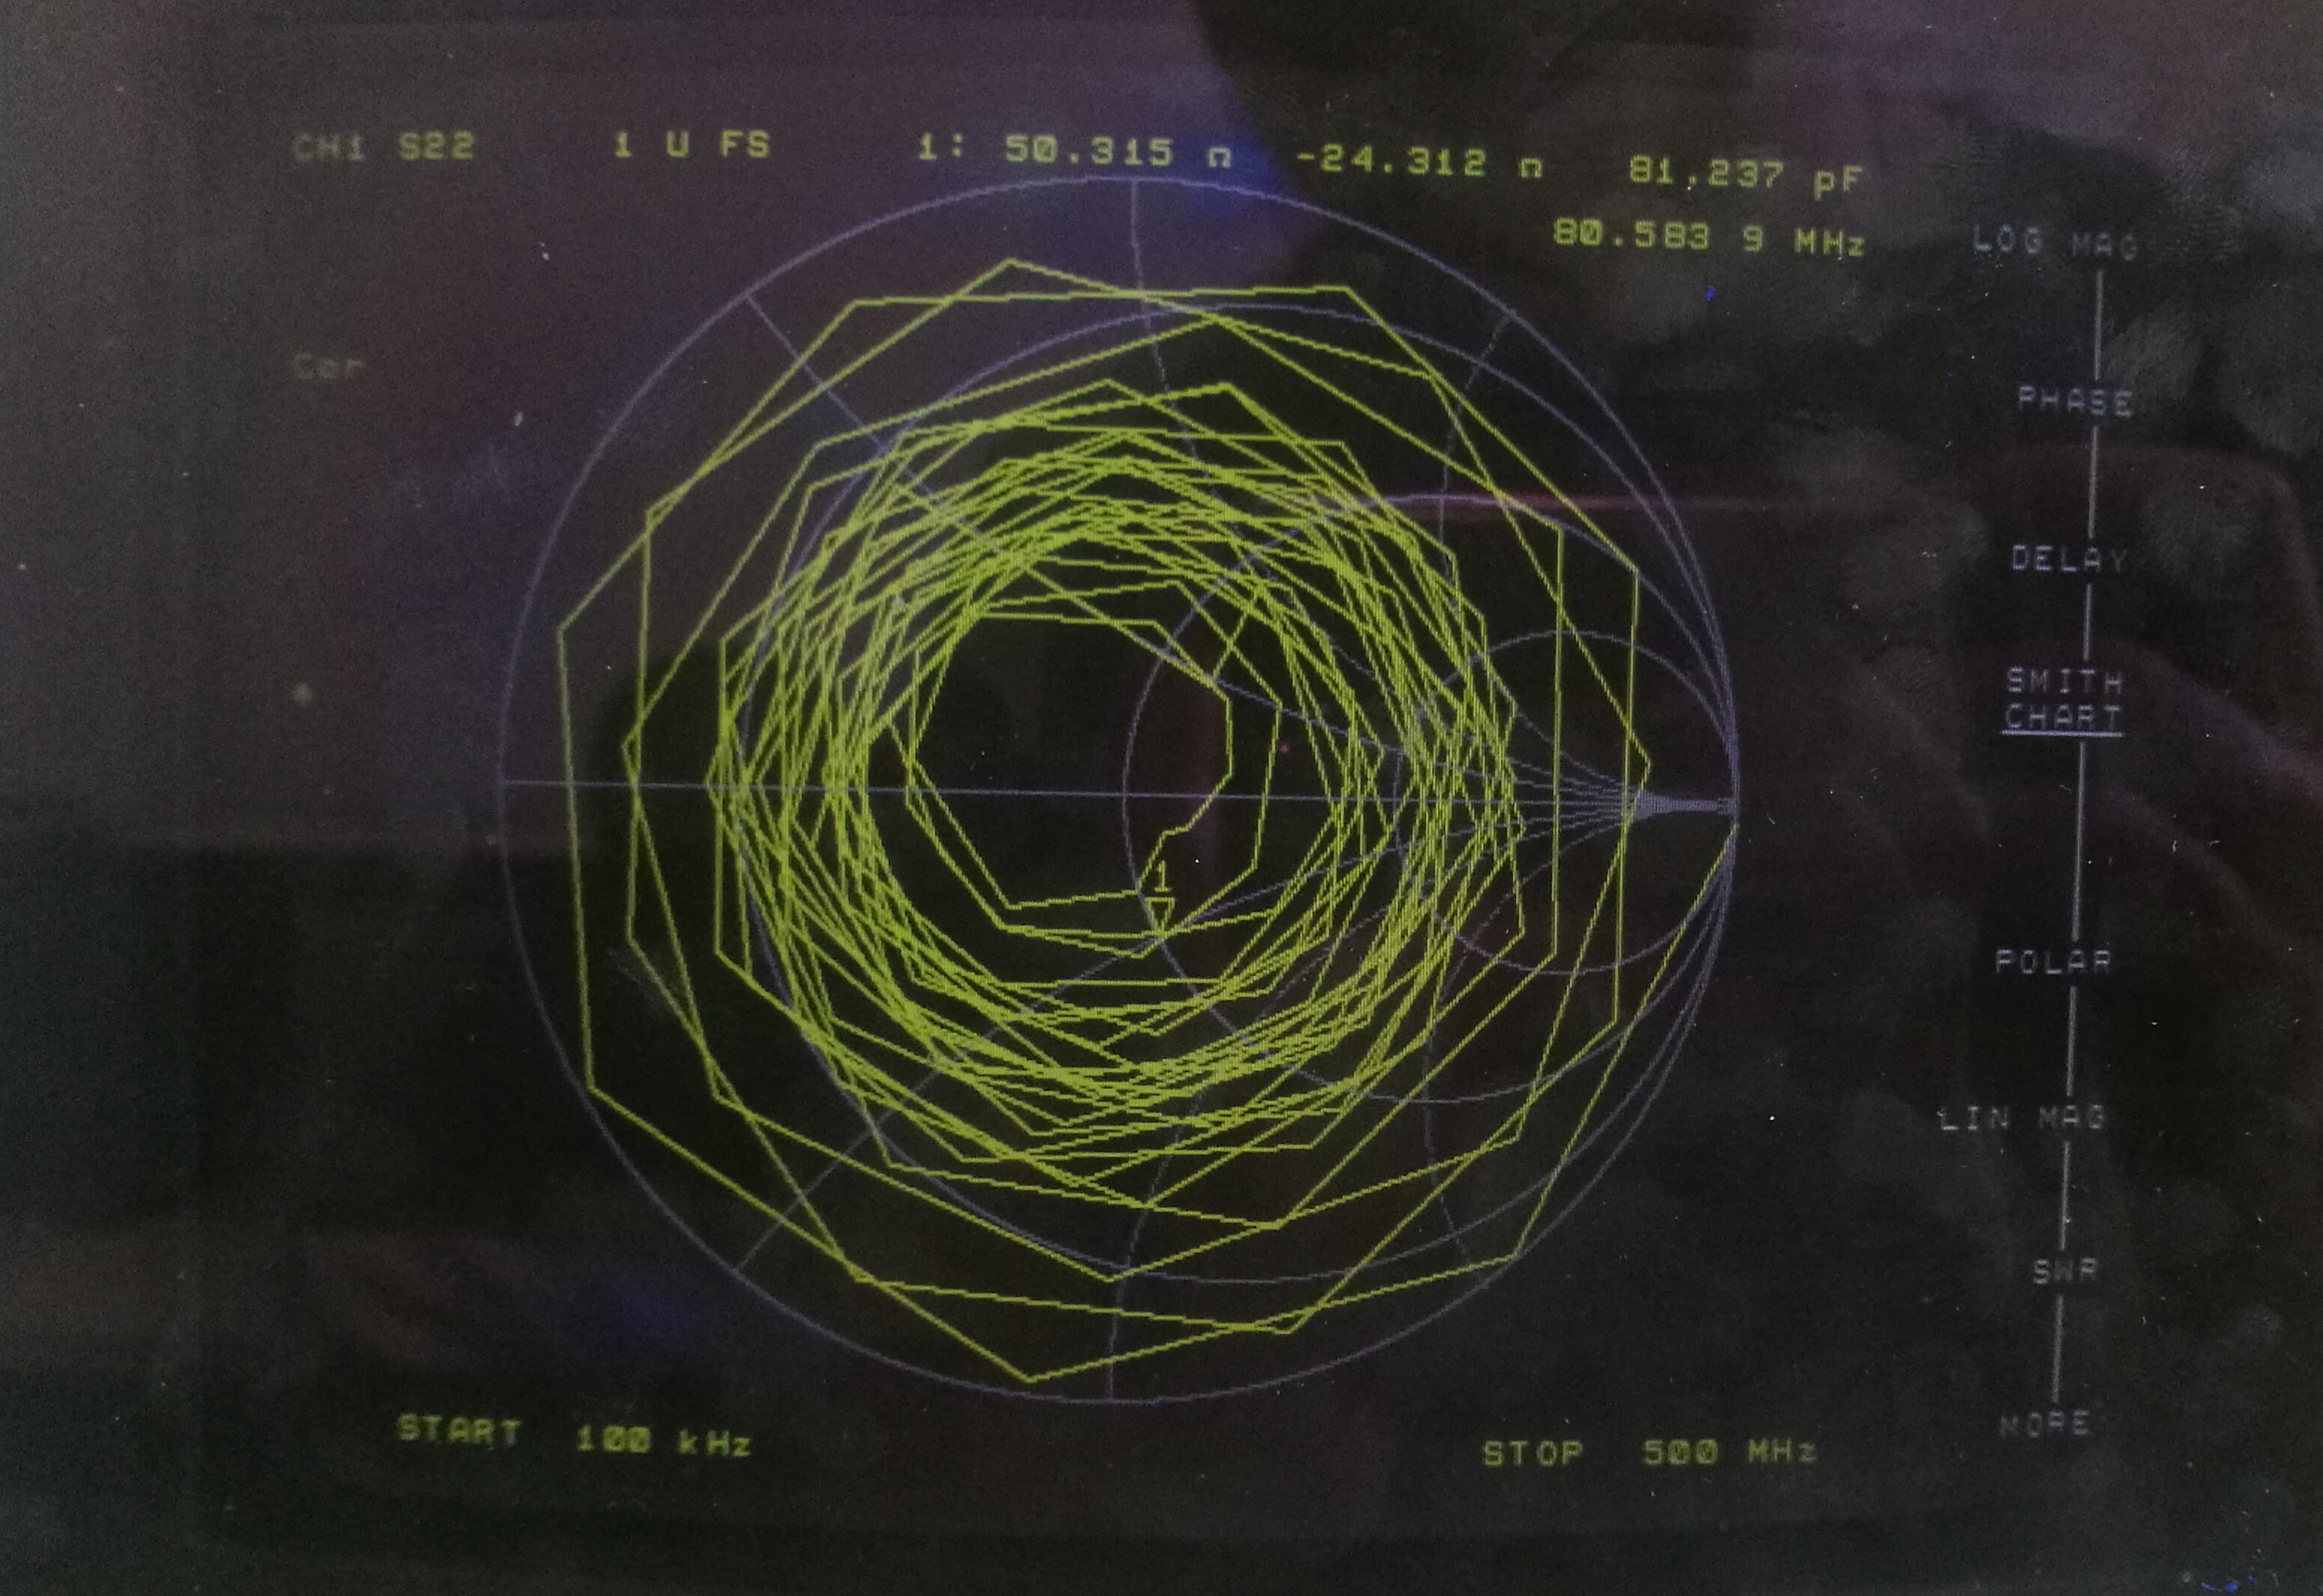
\includegraphics[scale = 0.065]{pic/Smith_grande.jpg} 
\end{center}

\chapter{Reception FM}
\addcontentsline{toc}{chapter}{Reception FM}

\chapter{Conclusion}
\addcontentsline{toc}{chapter}{Conclusion}

\end{document}